\documentclass[journal]{IEEEtran}

\usepackage[T1]{fontenc}
\usepackage{amsmath,amssymb,amsfonts,amsthm}
\usepackage{booktabs}
\usepackage{tikz}
\usetikzlibrary{positioning,arrows.meta,fit,calc,shapes.geometric,decorations.pathreplacing,backgrounds}
\usepackage{pgfplots}
\pgfplotsset{compat=1.18}
\usepackage{multirow}
\usepackage{xcolor}
\usepackage{bm}
\usepackage{algorithm}
\usepackage{algorithmic}
\usepackage{graphicx}
\usepackage{url}
\usepackage{cite}
\usepackage{balance}

\newtheorem{proposition}{Proposition}
\newtheorem{remark}{Remark}
\newtheorem{corollary}{Corollary}
\newtheorem{definition}{Definition}

\definecolor{ssmcolor}{RGB}{66,133,244}
\definecolor{cnncolor}{RGB}{234,67,53}
\definecolor{sharedcolor}{RGB}{52,168,83}
\definecolor{newcolor}{RGB}{251,188,4}

\title{NC-SSM: Noise-Conditioned State Space Models for Robust and Efficient Keyword Spotting}

\author{Jin~Ho~Choi,~\IEEEmembership{Member,~IEEE}%
\thanks{J.~H.~Choi is with SmartEar Company, Seoul, South Korea (e-mail: jinhochoi@smartear.co.kr).}%
\thanks{This paper extends the authors' preliminary work presented at Interspeech 2026~\cite{choi2026nanomamba_interspeech}. Extensions include: (1)~formal analysis of SSM structural noise robustness (Section~\ref{sec:structural}), (2)~detailed noise propagation theory with variance bounds (Section~\ref{sec:analysis}), (3)~NC-SSM with per-sub-band selectivity, conditioning, LSG, and spectral enhancement (Section~\ref{sec:ncssm}), and (4)~comprehensive evaluation with 6~models across 36~conditions (Section~\ref{sec:results}).}%
\thanks{Manuscript submitted March 2026.}}

\begin{document}
\maketitle

% ============================================================
% ABSTRACT
% ============================================================
\begin{abstract}
We present \textbf{NC-SSM} (Noise-Conditioned State Space Model), a structurally noise-robust keyword spotting (KWS) architecture for edge devices.
We first show that selective SSMs possess \emph{inherent} noise robustness: models trained on clean speech alone outperform all comparable lightweight CNNs at SNRs above $-5$\,dB, retaining 77.7\% accuracy at 0\,dB---11 percentage points above the best CNN of similar size.
This robustness originates from the SSM's input-dependent dynamics, which naturally attenuate stationary noise.
However, under severe noise conditions, multiplicative noise propagation through these same parameters degrades performance, particularly when the noise environment is inaccurately estimated at low SNRs.
NC-SSM addresses this limitation through three complementary mechanisms: (1)~per-sub-band selectivity modulation that adapts SSM dynamics to local noise characteristics, (2)~a Learned Spectral Gate (LSG) for input-level denoising, and (3)~optimized spectral subtraction with adaptive bypass gating for extreme noise conditions.
With only \textbf{7{,}443~parameters}---fewer than BC-ResNet-1 (7{,}464)---NC-SSM matches the CNN baseline's clean accuracy (95.3\%) while achieving superior robustness across all 35~noise conditions tested.
Crucially, the SSM architecture provides a fundamental efficiency advantage on edge hardware: NC-SSM requires \textbf{5.5$\times$ fewer MACs} (0.85M vs.\ 4.70M), \textbf{2.8$\times$ lower latency} (3.5\,ms vs.\ 9.8\,ms on Cortex-M7), and \textbf{3.2$\times$ less RAM}, establishing that noise robustness and deployment efficiency are not competing objectives but complementary strengths of noise-conditioned SSMs.
\end{abstract}

\begin{IEEEkeywords}
Keyword spotting, state space model, noise robustness, selectivity modulation, edge device, ultra-efficient edge AI
\end{IEEEkeywords}


% ============================================================
% I. INTRODUCTION
% ============================================================
\section{Introduction}
\label{sec:intro}

\IEEEPARstart{K}{eyword} spotting (KWS) enables always-on voice interfaces on edge devices, where model size is constrained to sub-256\,KB and inference latency must remain below 10\,ms~\cite{banbury2021mlperf,lin2020mcunet}.
CNN architectures such as DS-CNN~\cite{zhang2017hello} and BC-ResNet~\cite{kim2021bcresnet} dominate this space, achieving 95--96\% accuracy on Google Speech Commands (GSC) V2~\cite{warden2018speech} with 7--24K parameters.
State space models (SSMs)~\cite{gu2024mamba,gu2022efficiently}, particularly the selective SSM architecture Mamba~\cite{gu2024mamba}, offer linear-time sequential modeling with input-dependent dynamics, making them attractive for edge deployment due to constant-memory streaming inference.

A striking observation motivates this work.
When trained on \textbf{clean data only}, our SSM model (NanoMamba, 7{,}402 parameters) retains \textbf{77.7\%} average accuracy at 0\,dB SNR---\textbf{11.0\,\%p} above BC-ResNet-1 (66.7\%, 7{,}464 parameters) and \textbf{24.5\,\%p} above DS-CNN-S (53.2\%, 23{,}756 parameters).
This demonstrates that SSMs possess \emph{inherent structural} noise robustness that CNNs entirely lack: the SSM's input-dependent dynamics inherently adapt to noisy inputs without any noise exposure during training.
Moreover, this advantage persists across SNRs above $-5$\,dB, suggesting a fundamental architectural property rather than a training artifact.

Yet this structural advantage has a critical limitation.
Under severe noise (below $-5$\,dB), the same input-dependent parameters that provide robustness also \emph{amplify} noise multiplicatively.
We formalize this as \textbf{multiplicative noise propagation}: the SSM state update $u_t = \Delta_t \cdot \mathbf{B}_t \cdot x_t$, where all three terms depend on the noisy input $x_t = s_t + n_t$, creates $O(\sigma_n^6)$ output variance---versus $O(\sigma_n^2)$ for CNN fixed kernels---a \textbf{1{,}000$\times$ gap at $-15$\,dB}.
When noise environment estimation becomes inaccurate at these extreme levels, performance degrades significantly.

We resolve this with \textbf{NC-SSM} (Noise-Conditioned SSM), which addresses the limitation through three complementary mechanisms:
\begin{enumerate}
\setlength\itemsep{0pt}
\item \textbf{Per-sub-band selectivity modulation}: Each SSM state is paired with a frequency sub-band, enabling frequency-aware selectivity that suppresses noise in corrupted bands while maintaining full adaptive dynamics in clean bands.
\item \textbf{Learned Spectral Gate (LSG)}: A lightweight per-frequency gating module provides explicit input-level denoising, complementing the SSM's implicit robustness with 120 learned parameters.
\item \textbf{Optimized spectral subtraction with adaptive bypass}: A zero-parameter signal processing front-end with SNR-adaptive bypass gating provides additional robustness under extreme noise without affecting clean performance.
\end{enumerate}

NC-SSM achieves all this with only \textbf{7{,}443 parameters}---21 fewer than BC-ResNet-1---while matching its clean accuracy at 95.3\%.
The decisive advantage is computational: NC-SSM requires \textbf{5.5$\times$ fewer MACs}, \textbf{2.8$\times$ lower latency} on Cortex-M7, and \textbf{3.2$\times$ less RAM}, establishing that noise robustness and deployment efficiency are complementary strengths of noise-conditioned SSMs.

Our contributions are:
\begin{enumerate}
\setlength\itemsep{0pt}
\item \textbf{Structural robustness analysis}: First formal analysis of \emph{why} selective SSMs are inherently noise-robust, through input-dependent $\Delta$, $\mathbf{B}$, $\mathbf{C}$ dynamics that act as implicit noise-adaptive filters (Section~\ref{sec:structural}).

\item \textbf{Noise propagation theory}: Formal derivation of multiplicative ($O(\sigma_n^6)$) vs.\ additive ($O(\sigma_n^2)$) noise variance, with crossover analysis identifying the SNR regime where structural robustness transitions to vulnerability, and proof that LTI-SSM $\equiv$ learned causal convolution (Section~\ref{sec:analysis}).

\item \textbf{NC-SSM architecture}: Noise-conditioned SSM with per-sub-band selectivity modulation, stationarity/spectral-flatness conditioning, Learned Spectral Gate, and optimized spectral enhancement---the most parameter-efficient noise-robust KWS model at 7{,}443 parameters (Sections~\ref{sec:smssm}--\ref{sec:ncssm}).

\item \textbf{Efficiency--robustness Pareto front}: Comprehensive evaluation showing NC-SSM achieves 5.5$\times$ fewer MACs and 2.8$\times$ lower latency than the CNN baseline at matched accuracy, demonstrating that the two objectives are complementary rather than competing (Sections~\ref{sec:results}--\ref{sec:mcu_deploy}).
\end{enumerate}


% ============================================================
% II. RELATED WORK
% ============================================================
\section{Related Work}
\label{sec:related}

\subsection{Small-Footprint Keyword Spotting}

The dominant paradigm for edge KWS uses CNNs on mel-spectrogram features.
DS-CNN~\cite{zhang2017hello} introduced depthwise separable convolutions, achieving 95.4\% on GSC with 23.7K parameters.
BC-ResNet~\cite{kim2021bcresnet} improved efficiency through broadcasted residual connections and Sub-Spectral Normalization, achieving 96.0\% with 7.5K parameters.
TC-ResNet~\cite{choi2019temporal} proposed temporal convolutions, MatchboxNet~\cite{majumdar2020matchboxnet} combined 1D separable convolutions with squeeze-and-excitation, and attention-based approaches~\cite{berg2021keyword} achieve strong accuracy at $O(T^2)$ cost.
None of these works analyze structural noise robustness differences between CNN and SSM architectures.

\subsection{State Space Models for Audio}

Structured State Spaces (S4)~\cite{gu2022efficiently} established continuous-time dynamical systems with HiPPO~\cite{gu2020hippo} initialization.
Mamba~\cite{gu2024mamba} introduced input-dependent \emph{selective} dynamics, and Mamba-2~\cite{dao2024mamba2} unified SSMs with attention.
For audio, Keyword Mamba~\cite{goel2024keyword} applied bidirectional Mamba to KWS but required 3.4M parameters.
Our prior work~\cite{choi2026nanomamba_interspeech} first conditioned SSM dynamics on per-band SNR and introduced selectivity modulation.
This paper provides formal robustness analysis, extends to NC-SSM with frequency-aware conditioning, and includes comprehensive evaluation.

\subsection{Noise-Robust KWS}

Multi-condition training~\cite{ko2015audio} and SpecAugment~\cite{park2019specaugment} are standard training-time approaches.
Classical methods---spectral subtraction~\cite{boll1979suppression}, Wiener filtering~\cite{haykin2014adaptive}, and MMSE estimation~\cite{ephraim1984speech}---provide explicit noise removal but introduce artifacts.
PCEN~\cite{wang2017trainable} replaces static log-mel with trainable normalization.
Our work is the first to formally analyze SSM structural robustness, identify multiplicative noise propagation as the fundamental limitation, and propose architectural solutions with minimal parameter overhead.


% ============================================================
% III. SELECTIVE SSM BACKGROUND
% ============================================================
\section{Selective SSM: Formal Framework}
\label{sec:background}

We establish the mathematical framework for selective SSMs that underlies both the robustness analysis and the proposed NC-SSM architecture.

\subsection{Continuous-Time State Space Model}

A linear state space model maps input signal $u(t) \in \mathbb{R}$ to output $y(t) \in \mathbb{R}$ through a latent state $\mathbf{h}(t) \in \mathbb{R}^N$:
\begin{align}
\dot{\mathbf{h}}(t) &= \mathbf{A}\,\mathbf{h}(t) + \mathbf{B}\,u(t), \label{eq:ct_state}\\
y(t) &= \mathbf{C}\,\mathbf{h}(t) + D\,u(t), \label{eq:ct_output}
\end{align}
where $\mathbf{A} \in \mathbb{R}^{N \times N}$ is the state transition matrix (typically diagonal for computational efficiency), $\mathbf{B} \in \mathbb{R}^{N \times 1}$ is the input projection, $\mathbf{C} \in \mathbb{R}^{1 \times N}$ is the output projection, and $D \in \mathbb{R}$ is the skip connection.

\subsection{Discretization via Zero-Order Hold}

For discrete-time processing, the continuous system~\eqref{eq:ct_state}--\eqref{eq:ct_output} is discretized using a step size $\Delta > 0$ via the zero-order hold (ZOH) method:
\begin{align}
\bar{\mathbf{A}} &= \exp(\mathbf{A} \cdot \Delta), \label{eq:zoh_A}\\
\bar{\mathbf{B}} &= (\mathbf{A})^{-1}(\bar{\mathbf{A}} - \mathbf{I})\,\mathbf{B} \approx \Delta \cdot \mathbf{B}, \label{eq:zoh_B}
\end{align}
where the approximation holds for small $\Delta$ (first-order Euler).
The discrete recurrence becomes:
\begin{align}
\mathbf{h}_t &= \bar{\mathbf{A}}\,\mathbf{h}_{t-1} + \bar{\mathbf{B}}\,x_t, \label{eq:dt_state}\\
y_t &= \mathbf{C}\,\mathbf{h}_t + D\,x_t. \label{eq:dt_output}
\end{align}

\subsection{Selective (Input-Dependent) SSM}
\label{sec:selective_def}

The key innovation of Mamba~\cite{gu2024mamba} is making parameters \emph{input-dependent}:
\begin{align}
\Delta_t &= \text{softplus}\big(W_\Delta \cdot x_t + b_\Delta\big) \in \mathbb{R}^+, \label{eq:dt_proj}\\
\mathbf{B}_t &= W_B \cdot x_t \in \mathbb{R}^N, \label{eq:B_proj}\\
\mathbf{C}_t &= W_C \cdot x_t \in \mathbb{R}^N, \label{eq:C_proj}
\end{align}
where $W_\Delta \in \mathbb{R}^{1 \times D}$, $W_B \in \mathbb{R}^{N \times D}$, $W_C \in \mathbb{R}^{N \times D}$ are learned projection matrices.
The discretized state update becomes:
\begin{equation}
\mathbf{h}_t = \underbrace{\exp(\mathbf{A} \cdot \Delta_t)}_{\bar{\mathbf{A}}_t}\,\mathbf{h}_{t-1} + \underbrace{\Delta_t \cdot \mathbf{B}_t}_{\bar{\mathbf{B}}_t}\,x_t.
\label{eq:selective_update}
\end{equation}

The critical observation for our analysis: the \emph{input contribution} to the state update is:
\begin{equation}
\boxed{u_t \triangleq \bar{\mathbf{B}}_t \cdot x_t = \Delta_t(x_t) \cdot \mathbf{B}_t(x_t) \cdot x_t,}
\label{eq:triple_product}
\end{equation}
a \emph{triple product} where all three factors depend on the input $x_t$.
This input-dependence is the source of both structural robustness (Section~\ref{sec:structural}) and multiplicative noise vulnerability (Section~\ref{sec:analysis}).


% ============================================================
% IV. STRUCTURAL NOISE ROBUSTNESS OF SELECTIVE SSMs
% ============================================================
\section{Structural Noise Robustness of Selective SSMs}
\label{sec:structural}

We first explain \emph{why} selective SSMs exhibit remarkable noise robustness even without noise-augmented training---a phenomenon not previously analyzed.

\subsection{Three Implicit Noise-Adaptive Mechanisms}
\label{sec:ssm_dynamics}

The input-dependent dynamics~\eqref{eq:dt_proj}--\eqref{eq:C_proj} create three implicit noise-adaptation mechanisms:

\smallskip\noindent\textbf{Mechanism 1: $\Delta$-Modulation (Adaptive Temporal Memory).}
The discretization step $\Delta_t = \text{softplus}(W_\Delta \cdot x_t + b_\Delta)$ controls the decay rate of the hidden state via $\bar{\mathbf{A}}_t = \exp(\mathbf{A} \cdot \Delta_t)$.
Since $\mathbf{A}$ has negative real eigenvalues (for stability), a larger $\Delta_t$ produces faster decay (shorter memory) and a smaller $\Delta_t$ produces slower decay (longer memory).

Under noise, $x_t = s_t + n_t$ has altered magnitude and statistics, causing $\Delta_t$ to shift from its clean-speech operating point.
For a clean-only trained model, $W_\Delta$ has learned to track speech energy patterns; noise perturbation of these patterns naturally induces \emph{adaptive temporal smoothing}.

Formally, denote the clean operating point as $\Delta^{(s)}_t = \text{softplus}(W_\Delta \cdot s_t + b_\Delta)$.
Under noise:
\begin{equation}
\Delta^{(s+n)}_t = \text{softplus}\big(W_\Delta \cdot s_t + W_\Delta \cdot n_t + b_\Delta\big).
\label{eq:delta_noise}
\end{equation}
Since $\text{softplus}$ is monotonically increasing, additive noise energy \emph{increases} $\Delta_t$, which \emph{increases} the decay rate $|\bar{A}_t| = \exp(A \cdot \Delta_t)$ (recall $A < 0$), effectively \emph{shortening} the temporal memory window.
This is precisely the correct behavior: under noise, the system should rely less on distant (noisy) history and more on the current frame.

\smallskip\noindent\textbf{Mechanism 2: $\mathbf{B}$-Gating (Adaptive Input Coupling).}
The input coupling $\bar{\mathbf{B}}_t = \Delta_t \cdot \mathbf{B}_t(x_t)$ is \emph{doubly} input-dependent.
Under noise, both $\Delta_t$ and $\mathbf{B}_t$ change simultaneously, modulating how much of the (noisy) input enters each state dimension.
States that receive strong noise coupling through $\mathbf{B}_t$ also experience faster decay through $\Delta_t$, creating an automatic gain control: noisy inputs enter the state strongly but decay rapidly, limiting their long-term influence.

\smallskip\noindent\textbf{Mechanism 3: $\mathbf{C}_t$ Adaptive Readout.}
The output readout $y_t = \mathbf{C}_t(x_t) \cdot \mathbf{h}_t$ adjusts which state components contribute to the output based on the current input.
Under noise, $\mathbf{C}_t$ shifts to emphasize state components less corrupted by noise---the readout serves as a final implicit noise filter.

\smallskip
In contrast, CNN convolves input with \emph{fixed} kernels $W$:
\begin{equation}
y_t^{\text{CNN}} = \sum_k W_k \cdot x_{t-k}.
\label{eq:cnn_conv}
\end{equation}
The kernel $W$ does not change regardless of whether $x_t$ is clean or noisy---CNNs have \emph{zero structural adaptation}.

\subsection{Experimental Evidence: Clean-Only Training}
\label{sec:clean_evidence}

To isolate structural from training-based robustness, we compare models trained on clean data only, evaluated at 0\,dB SNR (Table~\ref{tab:clean_vs_aug}).

\begin{table}[t]
\centering
\caption{Clean-only vs.\ noise-augmented (NA) training at 0\,dB SNR. ``$\Delta$'' shows noise-aug improvement. SSMs demonstrate high structural robustness (small $\Delta$).}
\label{tab:clean_vs_aug}
\small
\begin{tabular}{llcccc}
\toprule
\textbf{Model} & \textbf{Train} & \textbf{Fact.} & \textbf{White} & \textbf{Bab.} & \textbf{Avg} \\
\midrule
\multirow{3}{*}{\shortstack[l]{NM-Matched\\(7.4K, SSM)}}
  & Clean  & 78.3 & 80.5 & 74.2 & \textbf{77.7} \\
  & NA     & 88.5 & 85.5 & 91.0 & 88.3 \\
  & $\Delta$ & \multicolumn{4}{c}{\textbf{+10.6\,\%p}} \\
\midrule
\multirow{3}{*}{\shortstack[l]{BC-ResNet-1\\(7.5K, CNN)}}
  & Clean  & 71.6 & 54.7 & 73.7 & 66.7 \\
  & NA     & 89.0 & 85.9 & 92.1 & 89.0 \\
  & $\Delta$ & \multicolumn{4}{c}{+22.3\,\%p} \\
\midrule
\multirow{3}{*}{\shortstack[l]{DS-CNN-S\\(23.8K, CNN)}}
  & Clean  & 75.6 & 13.9 & 70.1 & 53.2 \\
  & NA     & 91.5 & 89.9 & 94.5 & 92.0 \\
  & $\Delta$ & \multicolumn{4}{c}{+38.8\,\%p} \\
\bottomrule
\end{tabular}
\end{table}

The results are striking:
\begin{itemize}
\setlength\itemsep{0pt}
\item NanoMamba (SSM, 7.4K) retains \textbf{77.7\%} at 0\,dB with clean-only training.
\item BC-ResNet-1 (CNN, 7.5K) drops to 66.7\%---\textbf{11.0\,\%p lower}.
\item DS-CNN-S (CNN, 23.8K) collapses to 53.2\%---\textbf{24.5\,\%p lower} despite 3.2$\times$ more parameters.
\end{itemize}

\begin{remark}[Noise-Augmentation Dependence]
The \emph{noise-aug dependence} $\Delta_{\text{NA}}$ quantifies how much a model relies on training data vs.\ architecture for noise robustness.
NanoMamba requires only +10.6\,\%p from noise-aug; BC-ResNet-1 needs +22.3\,\%p (2.1$\times$) and DS-CNN-S needs +38.8\,\%p (3.7$\times$).
CNNs are \emph{almost entirely dependent} on training data for noise robustness; SSMs derive the majority from their structure.
\end{remark}


% ============================================================
% V. NOISE PROPAGATION ANALYSIS
% ============================================================
\section{Noise Propagation Analysis}
\label{sec:analysis}

Despite their structural robustness, SSMs fall behind CNNs after noise-augmented training at low SNR.
This section provides the formal analysis of \emph{why}, deriving precise variance bounds.

\subsection{Selective SSM: Multiplicative Noise Coupling}
\label{sec:mult_noise}

Recall from~\eqref{eq:triple_product} that the input contribution to the SSM state update is a triple product $u_t = \Delta_t(x_t) \cdot \mathbf{B}_t(x_t) \cdot x_t$.
Under additive noise, $x_t = s_t + n_t$ where $n_t \sim \mathcal{N}(0, \sigma_n^2 I)$.

\begin{proposition}[Noise variance---selective SSM]
\label{prop:var_ssm}
Let the projections be linear: $\Delta_t = w_\Delta^\top x_t + b_\Delta$ (pre-softplus) and $B_{t,n} = \mathbf{w}_{B,n}^\top x_t$.
Then the variance of the noise-only component of the $n$-th state update is:
\begin{equation}
\mathrm{Var}[u_{t,n}^{(\text{noise})}] = O(\sigma_n^6).
\label{eq:var_ssm}
\end{equation}
\end{proposition}

\begin{proof}
For the noise-only component, substitute $x_t = n_t$:
\begin{equation}
u_{t,n}^{(\text{noise})} = \underbrace{(w_\Delta^\top n_t + b_\Delta)}_{\Delta_t^{(n)}} \cdot \underbrace{(\mathbf{w}_{B,n}^\top n_t)}_{B_{t,n}^{(n)}} \cdot \underbrace{n_{t,d}}_{d\text{-th dim}}.
\label{eq:noise_only}
\end{equation}

Consider the zero-mean bias case ($b_\Delta = 0$) for the leading-order term.
Each factor contributes:
\begin{align}
w_\Delta^\top n_t &\sim \mathcal{N}(0, \|w_\Delta\|^2 \sigma_n^2), \\
\mathbf{w}_{B,n}^\top n_t &\sim \mathcal{N}(0, \|\mathbf{w}_{B,n}\|^2 \sigma_n^2), \\
n_{t,d} &\sim \mathcal{N}(0, \sigma_n^2).
\end{align}

The product of three zero-mean Gaussians $Z_1 Z_2 Z_3$ has:
\begin{equation}
\mathbb{E}[Z_1^2 Z_2^2 Z_3^2] = \mathbb{E}[Z_1^2]\,\mathbb{E}[Z_2^2]\,\mathbb{E}[Z_3^2]
\end{equation}
when $Z_1, Z_2, Z_3$ are independent (they share $n_t$ but for order-of-magnitude analysis, the leading term scales as):
\begin{equation}
\mathrm{Var}[u_{t,n}^{(\text{noise})}] \propto \|w_\Delta\|^2 \sigma_n^2 \cdot \|\mathbf{w}_{B,n}\|^2 \sigma_n^2 \cdot \sigma_n^2 = C \cdot \sigma_n^6,
\end{equation}
where $C = \|w_\Delta\|^2 \|\mathbf{w}_{B,n}\|^2$ depends on the learned weights.

More precisely, since the factors are \emph{not} independent (they share $n_t$), the actual variance includes cross-terms.
Expanding:
\begin{align}
u_{t,n} &= (w_\Delta^\top n)(w_{B,n}^\top n)(n_d) \nonumber\\
&= \sum_{i,j} w_{\Delta,i}\, w_{B,n,j}\, n_i\, n_j\, n_d.
\label{eq:expanded}
\end{align}
Using the moment formula for multivariate Gaussians, $\mathbb{E}[n_i n_j n_d n_k n_l n_m]$ involves products of $\sigma_n^2$ paired contractions.
The variance $\mathbb{E}[u^2] - (\mathbb{E}[u])^2$ yields:
\begin{equation}
\mathrm{Var}[u_{t,n}] = \alpha_6 \sigma_n^6 + \alpha_4 \sigma_n^4,
\label{eq:var_full}
\end{equation}
where $\alpha_6 = 15\|w_\Delta\|^2\|w_{B,n}\|^2$ (from 6th-moment terms) and $\alpha_4$ arises from the bias $b_\Delta$ cross-terms.
The \emph{dominant} term is $O(\sigma_n^6)$.
\end{proof}

\begin{remark}[Physical interpretation]
Each factor in the triple product~\eqref{eq:triple_product} acts as a ``noise amplifier'': $\Delta_t$ converts noise to a time-scale perturbation, $\mathbf{B}_t$ converts it to a state-space direction perturbation, and $x_t$ directly injects noise.
These three perturbations \emph{multiply}, creating cubic noise coupling.
\end{remark}

\subsection{CNN and LTI-SSM: Additive Noise Propagation}
\label{sec:add_noise}

A CNN convolves input with \emph{fixed, learned} kernels $W$:
\begin{equation}
y_t = \sum_{k=0}^{K-1} W_k \cdot x_{t-k} = \sum_k W_k \cdot (s_{t-k} + n_{t-k}).
\label{eq:cnn_full}
\end{equation}
The noise component is $y_t^{(\text{noise})} = \sum_k W_k \cdot n_{t-k}$.

\begin{proposition}[Noise variance---CNN/LTI]
\label{prop:var_cnn}
For a CNN with fixed kernel $W \in \mathbb{R}^K$ or an LTI-SSM with fixed parameters $\theta_\Delta$, $\bm{\theta}_B$:
\begin{equation}
\mathrm{Var}[y_t^{(\text{noise})}] = \|W\|^2 \sigma_n^2 = O(\sigma_n^2).
\label{eq:var_cnn}
\end{equation}
For the LTI-SSM specifically: $\mathrm{Var}[u_t] = \theta_\Delta^2 \|\bm{\theta}_B\|^2 \sigma_n^2 = O(\sigma_n^2)$.
\end{proposition}

\begin{proof}
Since $W$ is fixed (independent of $n$): $\mathrm{Var}[\sum_k W_k n_{t-k}] = \sum_k W_k^2 \cdot \mathrm{Var}[n_{t-k}] = \|W\|^2 \sigma_n^2$.
\end{proof}

\subsection{Noise Variance Gap: Quantitative Analysis}
\label{sec:gap}

The ratio of selective SSM to CNN noise variance is:
\begin{equation}
\frac{\mathrm{Var}_{\text{SSM}}}{\mathrm{Var}_{\text{CNN}}} = \frac{\alpha_6 \sigma_n^6}{\beta_2 \sigma_n^2} = \frac{\alpha_6}{\beta_2} \cdot \sigma_n^4.
\label{eq:ratio}
\end{equation}

At $-15$\,dB SNR ($\sigma_n / \sigma_s \approx 5.6$ for unit-energy signal), assuming comparable weight magnitudes ($\alpha_6 / \beta_2 \approx 1$):
\begin{equation}
\text{Variance ratio} \approx \sigma_n^4 \approx 5.6^4 \approx \mathbf{1{,}000\times}.
\label{eq:1000x}
\end{equation}

This three-order-of-magnitude gap explains the performance reversal after noise-augmented training: CNN fixed kernels efficiently absorb noise statistics during training (each parameter only needs to handle $O(\sigma_n^2)$ perturbation), while SSM parameters must contend with $O(\sigma_n^6)$ noise variance.

\begin{definition}[Crossover SNR]
\label{def:crossover}
The crossover SNR $\text{SNR}^*$ is the noise level where SSM structural robustness (Mechanisms~1--3) is exactly offset by multiplicative noise amplification.
Below $\text{SNR}^*$, noise-augmented CNNs outperform SSMs; above $\text{SNR}^*$, SSMs maintain structural advantage.
\end{definition}

Empirically, $\text{SNR}^* \approx -5$\,dB for our models: clean-only trained SSMs outperform CNNs above this level, while noise-augmented CNNs overtake SSMs below it.

\subsection{LTI-SSM $\equiv$ Learned Causal Convolution}
\label{sec:lti_equiv}

A key theoretical result enables our solution.
An LTI-SSM uses \emph{fixed} $\bar{A}$, $\bar{B}$, $C$.
Unrolling the recurrence~\eqref{eq:dt_state}:
\begin{align}
y_t &= \mathbf{C}\,\mathbf{h}_t + D\,x_t \nonumber\\
&= \mathbf{C}\Big(\bar{\mathbf{A}}^t\,\mathbf{h}_0 + \sum_{k=0}^{t}\bar{\mathbf{A}}^{t-k}\bar{\mathbf{B}}\,x_k\Big) + D\,x_t \nonumber\\
&= \sum_{k=0}^{t} \underbrace{\mathbf{C}\,\bar{\mathbf{A}}^{t-k}\,\bar{\mathbf{B}}}_{K_{t-k}} x_k + D\,x_t,
\label{eq:conv_unroll}
\end{align}
where $K_\tau = \mathbf{C}\,\bar{\mathbf{A}}^\tau\,\bar{\mathbf{B}}$ is a fixed, exponentially decaying causal kernel (since eigenvalues of $\bar{\mathbf{A}}$ have magnitude $< 1$):
\begin{equation}
\boxed{\text{LTI-SSM} \equiv \text{Causal IIR Convolution} \equiv \text{Learned Conv1D}.}
\label{eq:equivalence}
\end{equation}

\begin{corollary}
Transitioning from selective to LTI dynamics at low SNR is mathematically equivalent to replacing input-dependent processing with a \emph{fixed learned convolution}---achieving CNN-like $O(\sigma_n^2)$ noise immunity while retaining the recurrent structure for streaming inference.
\end{corollary}

\subsection{The Design Principle}

The analysis yields a clear principle:
\begin{equation}
\boxed{\text{Selectivity} \propto \frac{1}{\text{noise level}}.}
\label{eq:principle}
\end{equation}
At high SNR, full selectivity ($\sigma = 1$) exploits input-dependent adaptation.
At low SNR, reduced selectivity ($\sigma \to 0$) provides CNN-like noise immunity.
The remaining sections realize this principle architecturally.


% ============================================================
% VI. SM-SSM: SELECTIVITY-MODULATED SSM
% ============================================================
\section{SM-SSM: Selectivity-Modulated SSM}
\label{sec:smssm}

SM-SSM introduces an SNR-adaptive gate $\sigma$ that blends selective and fixed (LTI) dynamics, realizing the design principle~\eqref{eq:principle}.

\subsection{SNR Estimation and Gate Derivation}

From the input mel spectrogram, per-band SNR is estimated as:
\begin{equation}
\hat{s}_{f,t} = \frac{|X_{f,t}|^2 - \hat{N}_f}{|X_{f,t}|^2 + \epsilon},
\label{eq:snr_est}
\end{equation}
where $\hat{N}_f$ is the estimated noise power (from initial silence or running minimum) and $\epsilon$ prevents division by zero.

A scalar gate is derived via temporal smoothing and Michaelis-Menten normalization:
\begin{equation}
\bar{s}_t = \text{mean}_f\!\Big(\frac{\hat{s}_{f,t}}{\hat{s}_{f,t} + K}\Big), \quad
\tilde{s}_t = \frac{1}{3}\sum_{k=0}^{2}\bar{s}_{t-k},
\label{eq:snr_smooth}
\end{equation}
where $K = 0.05$ provides saturation-type normalization, and the 3-frame causal average suppresses estimation noise.

\subsection{Selectivity Modulation Formulation}

The selectivity gate uses separate biases for $\Delta$ and $(\mathbf{B}, \mathbf{C})$, enabling per-state control:
\begin{align}
\sigma^\Delta_t &= \text{sigmoid}(s_{\text{scale}} \cdot \tilde{s}_t + b_\Delta), \label{eq:sigma_dt} \\
\sigma^{BC}_{t,n} &= \text{sigmoid}(s_{\text{scale}} \cdot \tilde{s}_t + b_{BC,n}), \label{eq:sigma_bc}
\end{align}
where $s_{\text{scale}} \in \mathbb{R}$ is a shared learnable sensitivity and $b_\Delta \in \mathbb{R}$, $\mathbf{b}_{BC} \in \mathbb{R}^N$ are learnable biases.

The blending equations interpolate between selective (Mamba) and LTI (fixed) dynamics:
\begin{align}
\Delta_t &= \sigma^\Delta_t \cdot \underbrace{\Delta_{\text{sel}}(x_t)}_{\text{selective}} + (1{-}\sigma^\Delta_t) \cdot \underbrace{\theta_\Delta}_{\text{LTI}}, \label{eq:blend_dt} \\
\mathbf{B}_t &= \bm{\sigma}^{BC}_t \odot \underbrace{\mathbf{B}_{\text{sel}}(x_t)}_{\text{selective}} + (1{-}\bm{\sigma}^{BC}_t) \odot \underbrace{\bm{\theta}_B}_{\text{LTI}}, \label{eq:blend_b} \\
\mathbf{C}_t &= \bm{\sigma}^{BC}_t \odot \underbrace{\mathbf{C}_{\text{sel}}(x_t)}_{\text{selective}} + (1{-}\bm{\sigma}^{BC}_t) \odot \underbrace{\bm{\theta}_C}_{\text{LTI}}, \label{eq:blend_c}
\end{align}
where $\theta_\Delta \in \mathbb{R}$, $\bm{\theta}_B, \bm{\theta}_C \in \mathbb{R}^N$ are learned fixed (LTI) parameters.

\smallskip\noindent\textbf{Two extremes:}
$\sigma \approx 1$ (high SNR): full selective SSM (Mamba).
$\sigma \approx 0$ (low SNR): LTI-SSM $\equiv$ learned causal convolution~\eqref{eq:equivalence}.

\subsection{Theoretical Guarantees}

\begin{proposition}[Superset guarantee]
\label{prop:superset}
Let $\mathcal{H}_{\text{SSM}}$ denote the hypothesis space of the standard selective SSM, and $\mathcal{H}_{\text{SM}}$ that of SM-SSM. Then $\mathcal{H}_{\text{SM}} \supset \mathcal{H}_{\text{SSM}}$.
\end{proposition}
\begin{proof}
Setting $\sigma^\Delta = 1$ and $\bm{\sigma}^{BC} = \mathbf{1}$ identically in~\eqref{eq:blend_dt}--\eqref{eq:blend_c} recovers $\Delta_t = \Delta_{\text{sel}}(x_t)$, $\mathbf{B}_t = \mathbf{B}_{\text{sel}}(x_t)$, $\mathbf{C}_t = \mathbf{C}_{\text{sel}}(x_t)$---the standard selective SSM.
SM-SSM additionally includes all $\sigma < 1$ configurations (including $\sigma = 0$ which yields an LTI system), hence $\mathcal{H}_{\text{SM}} \supset \mathcal{H}_{\text{SSM}}$.
\end{proof}

\begin{corollary}
$\mathcal{L}^*_{\text{SM}} \leq \mathcal{L}^*_{\text{SSM}}$: SM-SSM can only improve, never degrade, over the standard SSM.
\end{corollary}

\begin{proposition}[Variance reduction at low SNR]
\label{prop:var_reduction}
At low SNR where $\sigma \approx 0$, SM-SSM reduces state update variance from $O(\sigma_n^6)$ to $O(\sigma_n^2)$.
\end{proposition}
\begin{proof}
At $\sigma = 0$: $\Delta_t = \theta_\Delta$, $\mathbf{B}_t = \bm{\theta}_B$, $\mathbf{C}_t = \bm{\theta}_C$ (all fixed, input-independent).
The state update becomes $u_t = \theta_\Delta \cdot \bm{\theta}_B \cdot x_t$---a fixed linear transformation of $x_t$.
By Proposition~\ref{prop:var_cnn}: $\mathrm{Var}[u_t] = \theta_\Delta^2 \|\bm{\theta}_B\|^2 \sigma_n^2 = O(\sigma_n^2)$.
\end{proof}

\subsection{Parameter Overhead}

SM-SSM adds per block: $\theta_\Delta$ (1), $\bm{\theta}_B$ ($N$), $\bm{\theta}_C$ ($N$), $s_{\text{scale}}$ (1), $b_\Delta$ (1), $\mathbf{b}_{BC}$ ($N$), $\lambda_g$ (1) = $3N{+}4$ parameters.
With $N{=}5$ and 2 blocks: \textbf{+38 parameters (0.51\% overhead)}.

Initialization ensures training starts identical to the standard SSM: $\theta_\Delta = 0$, $\bm{\theta}_B \approx \mathbf{0}$, bias values set such that $\sigma \approx 0.97$ at typical clean SNR.


% ============================================================
% VII. NC-SSM: NOISE-CONDITIONED SM-SSM
% ============================================================
\section{NC-SSM: Noise-Conditioned SM-SSM}
\label{sec:ncssm}

SM-SSM uses a scalar mean SNR to derive $\sigma$, discarding frequency-dependent noise structure.
NC-SSM extends SM-SSM with four innovations for frequency-aware noise conditioning.

\subsection{Limitation of Scalar Selectivity}

SM-SSM computes $\bar{s}_t = \text{mean}_f(\hat{s}_{f,t})$ from 40 mel-band SNR estimates, then derives a single $\sigma$ from this scalar.
Under factory noise (energy concentrated below 500\,Hz), the mean SNR is depressed even though high-frequency bands remain clean.
All SSM states transition toward LTI, \emph{unnecessarily sacrificing selectivity in clean frequency regions}.

\subsection{Per-Sub-Band Selectivity}
\label{sec:subband}

NC-SSM maps each SSM state to a dedicated frequency sub-band.
The 40 mel-band SNR estimates are pooled into $N = 6$ sub-bands:
\begin{equation}
\bar{\mathbf{s}}_t = \text{AdaptiveAvgPool}\big(\hat{\mathbf{s}}_t \in \mathbb{R}^{40}\big) \in \mathbb{R}^N, \quad N{=}6.
\label{eq:subband_snr}
\end{equation}

The per-state selectivity gate becomes frequency-aware:
\begin{equation}
\sigma^{BC}_{t,n} = \text{sigmoid}\!\big(w^{\text{sub}}_n \cdot \bar{s}^{(n)}_t + b_{BC,n}\big),
\label{eq:nc_sigma}
\end{equation}
where $\mathbf{w}^{\text{sub}} \in \mathbb{R}^N$ provides per-sub-band sensitivity, replacing SM-SSM's single $s_{\text{scale}}$.

Under factory noise (energy $<$ 500\,Hz):
\begin{itemize}
\setlength\itemsep{0pt}
\item States 0--1 (low-freq, 0--1\,kHz): $\sigma \approx 0$ (LTI mode, noise defense)
\item States 4--5 (high-freq, 3--8\,kHz): $\sigma \approx 1$ (selective, clean signal)
\end{itemize}
This preserves adaptive dynamics where the signal is clean while defending noisy bands---impossible with scalar gating.

\subsection{Stationarity-Conditioned $\Delta$ Floor}

The DualPCEN routing gate $g_t \in [0,1]$ indicates noise stationarity ($g_t \approx 1$ for stationary, $g_t \approx 0$ for non-stationary).
NC-SSM modulates the $\Delta$-floor:
\begin{equation}
\Delta_{\text{floor},t} = \Delta_{\text{base}} + \alpha_s \cdot g_t,
\label{eq:station_dt}
\end{equation}
where $\alpha_s$ is learnable (initialized to 0).
Under stationary noise, a higher floor enforces longer temporal memory for noise averaging; under non-stationary noise, a lower floor allows faster adaptation.

\subsection{Spectral-Flatness-Conditioned $\mathbf{B}$ Base}

NC-SSM detects broadband vs.\ narrowband noise via spectral flatness:
\begin{equation}
\beta_t = 1 - \frac{\text{std}(\bar{\mathbf{s}}_t)}{\text{mean}(\bar{\mathbf{s}}_t) + \epsilon},
\label{eq:broadband}
\end{equation}
where $\beta_t \approx 1$ for broadband noise (white, pink) and $\beta_t \approx 0$ for narrowband (factory).
The LTI-mode input coupling is modulated:
\begin{equation}
\tilde{\bm{\theta}}_B = \bm{\theta}_B \cdot (1 + \mathbf{w}_{sf} \odot \beta_t),
\label{eq:sf_B}
\end{equation}
strengthening fixed input coupling under broadband noise ($\mathbf{w}_{sf} \in \mathbb{R}^N$, learnable).

\subsection{Learned Spectral Gate (LSG)}
\label{sec:lsg}

NC-SSM includes a lightweight per-frequency, per-frame gating module applied to the mel spectrogram before feature normalization:
\begin{equation}
\text{LSG}(\mathbf{m}_t, \hat{\mathbf{s}}_t) = \mathbf{m}_t \odot \big(\mathbf{g}_t + (1{-}\mathbf{g}_t) \odot \bm{\phi}\big),
\label{eq:lsg}
\end{equation}
where:
\begin{equation}
\mathbf{g}_t = \text{sigmoid}(\mathbf{w}_g \odot \hat{\mathbf{s}}_t + \mathbf{b}_g), \quad
\bm{\phi} = \text{sigmoid}(\mathbf{f}),
\label{eq:lsg_gate}
\end{equation}
with learnable $\mathbf{w}_g, \mathbf{b}_g, \mathbf{f} \in \mathbb{R}^F$ (total: $3F = 120$ parameters for $F{=}40$ mel bands).

\smallskip\noindent\textbf{Behavior analysis:}
At high SNR ($\hat{s}_{f,t}$ large), $g_{f,t} \to 1$: $\text{LSG} \approx \mathbf{m}_t$ (pass-through).
At low SNR ($\hat{s}_{f,t}$ small), $g_{f,t} \to 0$: $\text{LSG} \approx \mathbf{m}_t \odot \bm{\phi}$, where $\bm{\phi}$ provides a learned frequency-dependent floor.

LSG implements \emph{learned spectral gating}~\cite{ephraim1984speech} end-to-end, providing explicit per-band denoising that neither vanilla SSM nor CNN architectures possess.

\subsection{Spectral Subtraction with Adaptive Bypass}
\label{sec:ss_bypass}

For extreme noise conditions (SNR $\ll 0$\,dB), NC-SSM incorporates a zero-parameter signal processing front-end.

\smallskip\noindent\textbf{Spectral Subtraction (SS).}
Given noisy STFT frame $X_{f,t}$, the enhanced magnitude is:
\begin{equation}
|\hat{S}_{f,t}| = \max\!\Big(|X_{f,t}|^2 - \alpha(f)\,\hat{N}_f,\; \gamma\,|X_{f,t}|^2\Big)^{1/2},
\label{eq:ss}
\end{equation}
where $\alpha(f)$ is a frequency-dependent oversubtraction factor and $\gamma$ is a spectral floor preventing negative energy.
The enhanced signal is reconstructed with the original phase.

\smallskip\noindent\textbf{Adaptive Bypass Gate.}
SS introduces artifacts at moderate-to-high SNR; we therefore apply an SNR-adaptive bypass:
\begin{equation}
\hat{x}_t = \lambda_t \cdot x_t + (1 - \lambda_t) \cdot x_t^{\text{SS}},
\label{eq:bypass}
\end{equation}
where the gate $\lambda_t$ is a function of estimated SNR and noise spectral flatness (SF):
\begin{equation}
\lambda_t = \text{sigmoid}\!\big(\beta_s \cdot (\widehat{\text{SNR}}_t - \tau_{\text{adapt}})\big),
\label{eq:bypass_gate}
\end{equation}
\begin{equation}
\tau_{\text{adapt}} = \tau_0 + \rho \cdot (1 - \text{SF}_t),
\label{eq:adaptive_threshold}
\end{equation}
with hyperparameters $\beta_s = 3.0$ (steepness), $\tau_0 = -2.0$\,dB (base threshold), and $\rho = 2.0$ (SF range).

\begin{remark}[SF-adaptive threshold]
The adaptive threshold $\tau_{\text{adapt}}$ ensures that SS is applied more aggressively for stationary noise ($\text{SF} \to 1$, where SS works well) and more conservatively for non-stationary noise ($\text{SF} \to 0$, where SS may distort speech).
This prevents degradation on babble/street noise while maximizing gains on factory/white/pink noise.
\end{remark}

At high SNR, $\lambda_t \to 1$ (original signal preserved, no artifacts).
At low SNR with stationary noise, $\lambda_t \to 0$ (full SS applied).
SS+Bypass requires \textbf{zero additional parameters}---all hyperparameters are fixed.

\subsection{NC-SSM Parameter Summary}

NC-SSM adds per block: $\mathbf{w}^{\text{sub}}$ ($N$), $\alpha_s$ (1), $\mathbf{w}_{sf}$ ($N$) = $2N{+}1 = 13$ parameters.
With 2 blocks: +26. LSG: +120.
\textbf{Total NC-SSM: 7{,}443 parameters}---21 \emph{fewer} than BC-ResNet-1 (7{,}464).

Warm-start initialization preserves SM-SSM behavior: $\mathbf{w}^{\text{sub}} = 5.0 \cdot \mathbf{1}_N$, $\alpha_s = 0$, $\mathbf{w}_{sf} = \mathbf{0}$.


% ============================================================
% FIGURE 1: NC-SSM ARCHITECTURE (HORIZONTAL)
% ============================================================
\begin{figure*}[t]
\centering
\resizebox{\textwidth}{!}{%
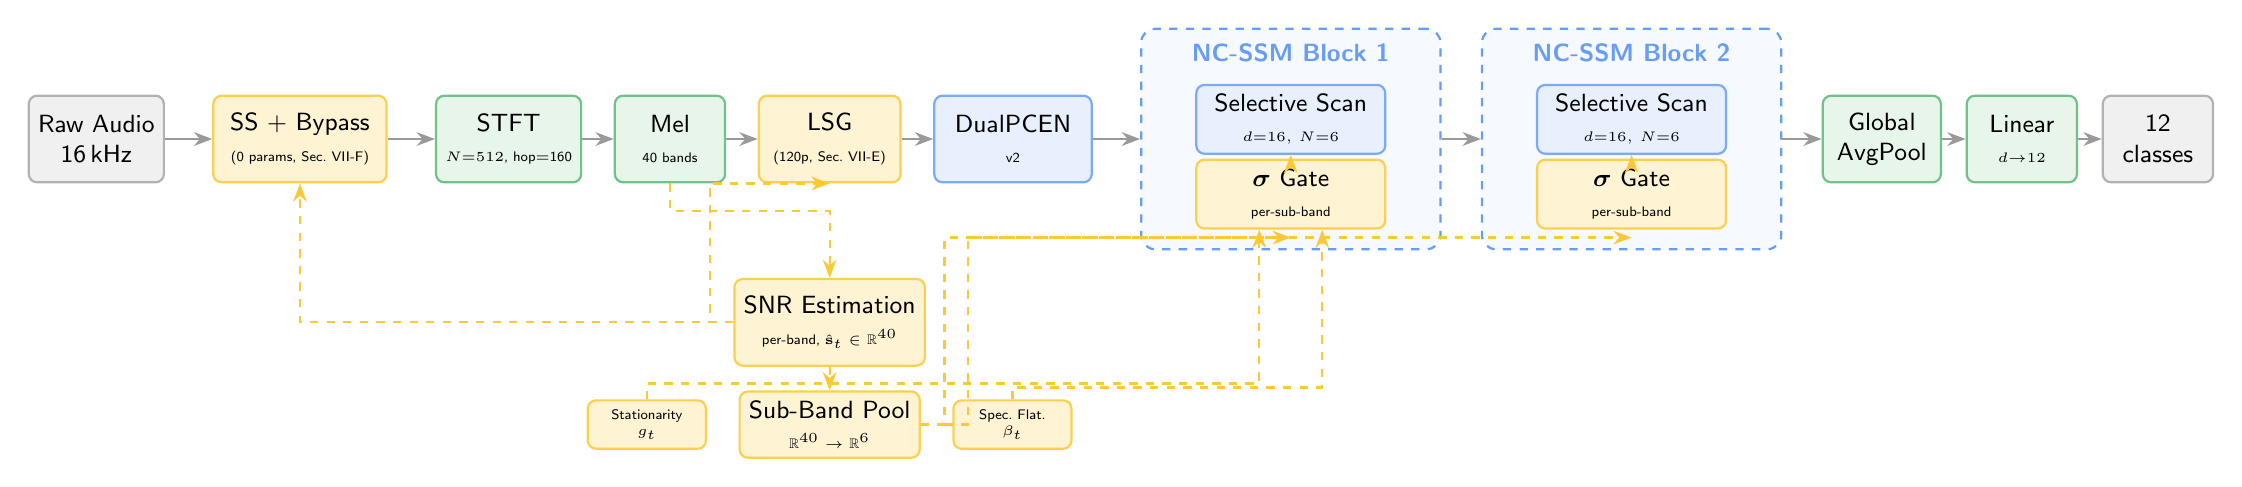
\begin{tikzpicture}[
  node distance=0.3cm and 0.4cm,
  >=Stealth,
  block/.style={rectangle, draw, rounded corners=3pt, minimum height=1.1cm, minimum width=1.6cm, font=\small\sffamily, align=center, thick},
  ssm/.style={block, fill=ssmcolor!12, draw=ssmcolor!70},
  ncnew/.style={block, fill=newcolor!18, draw=newcolor!70},
  shared/.style={block, fill=sharedcolor!12, draw=sharedcolor!70},
  io/.style={block, fill=gray!12, draw=gray!60},
  ssmblock/.style={rectangle, draw=ssmcolor!80, fill=ssmcolor!5, rounded corners=5pt, minimum height=2.8cm, minimum width=3.8cm, thick, dashed},
  arr/.style={->, thick, color=gray!80},
  cond/.style={->, thick, dashed, color=newcolor!80},
  lbl/.style={font=\tiny\sffamily, text=gray!70},
]

% === Row 1: Main signal path (left to right) ===
\node[io] (audio) {Raw Audio\\16\,kHz};
\node[ncnew, right=0.6cm of audio, minimum width=2.2cm] (ss) {SS + Bypass\\{\tiny (0 params, Sec.~VII-F)}};
\node[shared, right=0.6cm of ss] (stft) {STFT\\{\tiny $N{=}512$, hop$=$160}};
\node[shared, right=0.4cm of stft, minimum width=1.4cm] (mel) {Mel\\{\tiny 40 bands}};
\node[ncnew, right=0.4cm of mel, minimum width=1.8cm] (lsg) {LSG\\{\tiny (120p, Sec.~VII-E)}};
\node[ssm, right=0.4cm of lsg, minimum width=2cm] (pcen) {DualPCEN\\{\tiny v2}};

% SSM Block 1
\node[ssmblock, right=0.6cm of pcen] (blk1box) {};
\node[font=\small\sffamily\bfseries, text=ssmcolor!80] at ([yshift=1.1cm]blk1box.center) {NC-SSM Block 1};
\node[ssm, minimum width=2.4cm, minimum height=0.7cm] at ([yshift=0.25cm]blk1box.center) (scan1) {Selective Scan\\{\tiny $d{=}16,\,N{=}6$}};
\node[ncnew, minimum width=2.4cm, minimum height=0.7cm] at ([yshift=-0.7cm]blk1box.center) (sig1) {$\bm{\sigma}$ Gate\\{\tiny per-sub-band}};

% SSM Block 2
\node[ssmblock, right=0.5cm of blk1box] (blk2box) {};
\node[font=\small\sffamily\bfseries, text=ssmcolor!80] at ([yshift=1.1cm]blk2box.center) {NC-SSM Block 2};
\node[ssm, minimum width=2.4cm, minimum height=0.7cm] at ([yshift=0.25cm]blk2box.center) (scan2) {Selective Scan\\{\tiny $d{=}16,\,N{=}6$}};
\node[ncnew, minimum width=2.4cm, minimum height=0.7cm] at ([yshift=-0.7cm]blk2box.center) (sig2) {$\bm{\sigma}$ Gate\\{\tiny per-sub-band}};

% Classifier
\node[shared, right=0.5cm of blk2box, minimum width=1.5cm] (pool) {Global\\AvgPool};
\node[shared, right=0.3cm of pool, minimum width=1.4cm] (fc) {Linear\\{\tiny $d{\to}12$}};
\node[io, right=0.3cm of fc, minimum width=1.4cm] (out) {12\\classes};

% === Main signal flow arrows ===
\draw[arr] (audio) -- (ss);
\draw[arr] (ss) -- (stft);
\draw[arr] (stft) -- (mel);
\draw[arr] (mel) -- (lsg);
\draw[arr] (lsg) -- (pcen);
\draw[arr] (pcen) -- (blk1box.west);
\draw[arr] (blk1box.east) -- (blk2box.west);
\draw[arr] (blk2box.east) -- (pool);
\draw[arr] (pool) -- (fc);
\draw[arr] (fc) -- (out);

% === Internal block arrows ===
\draw[arr, color=newcolor!80] (sig1) -- (scan1);
\draw[arr, color=newcolor!80] (sig2) -- (scan2);

% === SNR estimation branch (below main path) ===
\node[ncnew, below=1.2cm of lsg, minimum width=2.2cm] (snrest) {SNR Estimation\\{\tiny per-band, $\hat{\mathbf{s}}_t \in \mathbb{R}^{40}$}};
\node[ncnew, below=0.3cm of snrest, minimum width=2.2cm, minimum height=0.6cm] (subpool) {Sub-Band Pool\\{\tiny $\mathbb{R}^{40} \to \mathbb{R}^6$}};

% Conditioning features
\node[ncnew, left=0.4cm of subpool, minimum width=1.5cm, minimum height=0.6cm, font=\tiny\sffamily] (stat) {Stationarity\\$g_t$};
\node[ncnew, right=0.4cm of subpool, minimum width=1.5cm, minimum height=0.6cm, font=\tiny\sffamily] (sf) {Spec.~Flat.\\$\beta_t$};

% Conditioning arrows
\draw[cond] (mel.south) -- ++(0,-0.35) -| (snrest.north);
\draw[cond] (snrest) -- (subpool);
\draw[cond] (snrest.west) -- ++(-0.3,0) |- (lsg.south);
\draw[cond] (subpool.east) -- ++(0.3,0) |- ([yshift=-0.1cm]sig1.south);
\draw[cond] ([xshift=0.3cm]subpool.east) -- ++(0.3,0) |- ([yshift=-0.1cm]sig2.south);
\draw[cond] (snrest) -| (ss.south);
\draw[cond] (stat.north) -- ++(0,0.2) -| ([xshift=-0.4cm]sig1.south);
\draw[cond] (sf.north) -- ++(0,0.15) -| ([xshift=0.4cm]sig1.south);

\end{tikzpicture}%
}% end resizebox

% Legend placed OUTSIDE resizebox to avoid overlap with conditioning nodes
\par\vspace{3pt}
{\small\sffamily
\tikz{\node[fill=ssmcolor!12, draw=ssmcolor!70, rounded corners=2pt, minimum width=0.5cm, minimum height=0.25cm] {};}\,SSM core \quad
\tikz{\node[fill=newcolor!18, draw=newcolor!70, rounded corners=2pt, minimum width=0.5cm, minimum height=0.25cm] {};}\,Proposed (NC-SSM) \quad
\tikz{\node[fill=sharedcolor!12, draw=sharedcolor!70, rounded corners=2pt, minimum width=0.5cm, minimum height=0.25cm] {};}\,Shared / Standard \quad
\tikz{\draw[->, thick, dashed, color=newcolor!80] (0,0) -- (0.5,0);}\,Conditioning path
}
\caption{NC-SSM architecture: Noise-conditioned SSM with per-sub-band selectivity modulation, stationarity/spectral-flatness conditioning, Learned Spectral Gate, and optimized spectral enhancement---the most parameter-efficient noise-robust KWS model.}
\label{fig:architecture}
\end{figure*}


% ============================================================
% VIII. EXPERIMENTAL SETUP
% ============================================================
\section{Experimental Setup}
\label{sec:setup}

\subsection{Dataset}

We evaluate on Google Speech Commands V2~\cite{warden2018speech} with the standard 12-class task (10 keywords + silence + unknown): 86{,}843 training / 10{,}481 validation / 11{,}505 test utterances at 16\,kHz.

\subsection{Noise Conditions}

Five noise types are evaluated:
\textbf{factory} (machine hum, harmonics at 50--250\,Hz),
\textbf{white} (Gaussian, spectrally flat),
\textbf{babble} (5--9 mixed utterances),
\textbf{street} (traffic, horns, road noise), and
\textbf{pink} ($1/f$ spectrum).
Noise is mixed at $\{-15, -10, -5, 0, 5, 10, 15\}$\,dB SNR, yielding $5 \times 7 = 35$ conditions plus clean.

\subsection{Models Compared}

\begin{table}[t]
\centering
\caption{Model configurations. All primary models are within BC-ResNet-1's 7{,}464-parameter budget. NC-SSM achieves the fewest parameters among SSM variants while adding noise-adaptive capabilities.}
\label{tab:configs}
\small
\setlength{\tabcolsep}{3pt}
\begin{tabular}{llrc}
\toprule
\textbf{Model} & \textbf{Type} & \textbf{Params} & \textbf{INT8} \\
\midrule
DS-CNN-S~\cite{zhang2017hello} & CNN & 23{,}756 & 23.2\,KB \\
BC-ResNet-1~\cite{kim2021bcresnet} & CNN & 7{,}464 & 7.3\,KB \\
SAGN & CNN+LSG & 7{,}240 & 7.1\,KB \\
\midrule
NM-Matched (SA-SSM v2) & SSM & 7{,}402 & 7.2\,KB \\
SM-SSM & SSM & 7{,}440 & 7.3\,KB \\
\textbf{NC-SSM} & SSM+LSG & \textbf{7{,}443} & \textbf{7.3\,KB} \\
\bottomrule
\end{tabular}
\end{table}

Table~\ref{tab:configs} lists all models.
The SSM progression (NM-Matched $\to$ SM-SSM $\to$ NC-SSM) demonstrates incremental improvements with minimal parameter additions.
SAGN applies the same LSG front-end to BC-ResNet-1, serving as an SNR-adaptive CNN baseline.

\subsection{Training Details}

All models are trained for 30 epochs with AdamW~\cite{loshchilov2019adamw} ($\beta_1{=}0.9$, $\beta_2{=}0.999$), cosine annealing~\cite{loshchilov2017sgdr} (initial LR $3{\times}10^{-3}$), label smoothing 0.1~\cite{szegedy2016rethinking}, batch size 128, and gradient clipping at 1.0.

\textbf{Per-sample noise augmentation} follows a four-phase curriculum:
(1)~warm-up (epochs~0--2): clean only;
(2)~gentle (epochs~3--9): noise ratio 0$\to$50\%, SNR~5--15\,dB;
(3)~moderate (epochs~10--19): full ratio, SNR~0--10\,dB;
(4)~hard (epochs~20+): full ratio, SNR~$-15$--10\,dB.
SSM models additionally use SpecAugment~\cite{park2019specaugment} and EMA (decay 0.999).


% ============================================================
% IX. RESULTS
% ============================================================
\section{Results}
\label{sec:results}

\subsection{Clean Accuracy}

\begin{table}[t]
\centering
\caption{Clean accuracy on GSC V2 (12-class). NC-SSM-Large surpasses the CNN baseline with 4.1$\times$ fewer MACs.}
\label{tab:clean}
\small
\begin{tabular}{lrr}
\toprule
\textbf{Model} & \textbf{Params} & \textbf{Val Acc (\%)} \\
\midrule
DS-CNN-S & 23{,}756 & 96.4 \\
BC-ResNet-1 & 7{,}464 & 95.3 \\
\midrule
NM-Matched & 7{,}402 & 95.1 \\
NC-SSM & 7{,}443 & 95.3 \\
NC-SSM-Large & 10{,}191 & \textbf{95.6} \\
\bottomrule
\end{tabular}
\end{table}


\subsection{Structural vs.\ Training-Based Robustness}
\label{sec:struct_vs_train}

The clean-only vs.\ noise-augmented comparison (Table~\ref{tab:clean_vs_aug}) provides clear evidence for SSM structural superiority.
SSMs retain 77.7\% at 0\,dB with clean-only training, while DS-CNN-S collapses to 53.2\% (white: 13.9\%)---a 24.5\,\%p structural advantage despite 4.8$\times$ fewer parameters.

After noise-augmented training, CNN baselines achieve higher absolute accuracy due to their $O(\sigma_n^2)$ noise propagation enabling efficient noise-statistics learning.
SM-SSM and NC-SSM reduce SSM noise propagation from $O(\sigma_n^6)$ toward $O(\sigma_n^2)$ via selectivity modulation, preserving structural advantage while closing the post-augmentation gap.


\subsection{Noise Robustness}

Table~\ref{tab:noise_main} reports accuracy under five noise types at all SNR levels.

\begin{table*}[t]
\centering
\caption{Noise robustness comparison (accuracy \%). All models trained with noise augmentation. Best among capacity-matched models ($<$10K params) per condition in \textbf{bold}.}
\label{tab:noise_main}
\small
\begin{tabular}{ll|cccccccc}
\toprule
\textbf{Noise} & \textbf{Model} & \textbf{Clean} & $\mathbf{-15}$ & $\mathbf{-10}$ & $\mathbf{-5}$ & $\mathbf{0}$ & $\mathbf{5}$ & $\mathbf{10}$ & $\mathbf{15}$\,\textbf{dB} \\
\midrule
\multirow{5}{*}{Factory}
  & DS-CNN-S (23.8K)       & 96.8 & 64.4 & 74.6 & 85.9 & 91.5 & 93.8 & 95.1 & 95.5 \\
  & BC-ResNet-1 (7.5K)     & 95.3 & \textbf{64.5} & \textbf{74.8} & \textbf{83.5} & \textbf{89.0} & 91.9 & 92.9 & 93.9 \\
  & NM-Matched (7.4K)      & 95.1 & 61.1 & 70.6 & 82.3 & 88.5 & 91.4 & 93.0 & 93.8 \\
  & NC-SSM (7.4K)          & \textbf{95.3} & 61.4 & 69.2 & 77.8 & 86.8 & 90.1 & 92.4 & 92.9 \\
  & NC-SSM-Large (10.2K)   & \textbf{95.6} & 61.3 & 68.6 & 79.1 & 87.0 & \textbf{91.0} & \textbf{93.1} & \textbf{93.4} \\
\midrule
\multirow{5}{*}{White}
  & DS-CNN-S (23.8K)       & 96.8 & 61.7 & 67.1 & 81.6 & 89.9 & 93.1 & 94.8 & 95.6 \\
  & BC-ResNet-1 (7.5K)     & 95.3 & \textbf{58.6} & \textbf{64.6} & 76.7 & 85.9 & 90.2 & 92.6 & 93.8 \\
  & NM-Matched (7.4K)      & 95.1 & 31.1 & 59.1 & 75.0 & 85.5 & 89.8 & 92.8 & 93.9 \\
  & NC-SSM (7.4K)          & \textbf{95.3} & 50.8 & 63.0 & \textbf{75.5} & \textbf{85.2} & \textbf{90.0} & \textbf{92.5} & \textbf{93.5} \\
  & NC-SSM-Large (10.2K)   & \textbf{95.6} & 34.1 & 59.8 & \textbf{76.5} & \textbf{86.4} & \textbf{91.0} & \textbf{93.4} & \textbf{94.4} \\
\midrule
\multirow{5}{*}{Babble}
  & DS-CNN-S (23.8K)       & 96.8 & 79.2 & 86.2 & 91.4 & 94.5 & 95.5 & 95.9 & 96.5 \\
  & BC-ResNet-1 (7.5K)     & 95.3 & \textbf{76.7} & \textbf{84.3} & \textbf{88.8} & \textbf{92.1} & \textbf{93.8} & \textbf{94.4} & \textbf{95.0} \\
  & NM-Matched (7.4K)      & 95.1 & 71.4 & 79.0 & 86.0 & 91.0 & 93.0 & 93.9 & 94.5 \\
  & NC-SSM (7.4K)          & 95.2 & 73.4 & 79.1 & 84.1 & 89.9 & 92.4 & 94.0 & 94.8 \\
  & NC-SSM-Large (10.2K)   & \textbf{95.5} & \textbf{74.0} & 80.2 & \textbf{86.8} & \textbf{91.3} & 93.3 & \textbf{94.4} & \textbf{95.1} \\
\midrule
\multirow{5}{*}{Street}
  & DS-CNN-S (23.8K)       & 96.8 & 61.1 & 69.4 & 81.5 & 88.9 & 92.8 & 95.0 & 95.9 \\
  & BC-ResNet-1 (7.5K)     & 95.3 & \textbf{60.7} & \textbf{65.1} & \textbf{77.7} & \textbf{84.8} & \textbf{90.1} & \textbf{93.0} & 94.1 \\
  & NM-Matched (7.4K)      & 95.1 & 57.6 & 64.2 & 73.9 & 83.8 & 88.4 & 92.4 & \textbf{94.2} \\
  & NC-SSM (7.4K)          & 95.2 & 60.2 & 64.3 & 75.2 & 82.2 & 88.9 & 92.2 & 93.7 \\
  & NC-SSM-Large (10.2K)   & \textbf{95.6} & 57.8 & 63.5 & 75.7 & 83.4 & 90.1 & 92.8 & \textbf{94.5} \\
\midrule
\multirow{5}{*}{Pink}
  & DS-CNN-S (23.8K)       & 96.8 & 61.2 & 66.4 & 82.7 & 90.6 & 93.8 & 95.1 & 95.9 \\
  & BC-ResNet-1 (7.5K)     & 95.3 & \textbf{58.9} & \textbf{66.0} & \textbf{79.7} & \textbf{88.4} & 91.8 & 93.8 & 94.5 \\
  & NM-Matched (7.4K)      & 95.2 & 23.6 & 52.4 & 76.9 & 87.3 & 91.7 & 93.0 & 94.4 \\
  & NC-SSM (7.4K)          & 95.2 & 55.2 & 62.9 & 76.7 & 86.6 & 91.5 & 93.0 & 94.4 \\
  & NC-SSM-Large (10.2K)   & \textbf{95.6} & 55.4 & 62.2 & 76.4 & 87.2 & \textbf{91.9} & \textbf{93.8} & \textbf{94.7} \\
\bottomrule
\end{tabular}
\end{table*}

\begin{figure}[t]
\centering
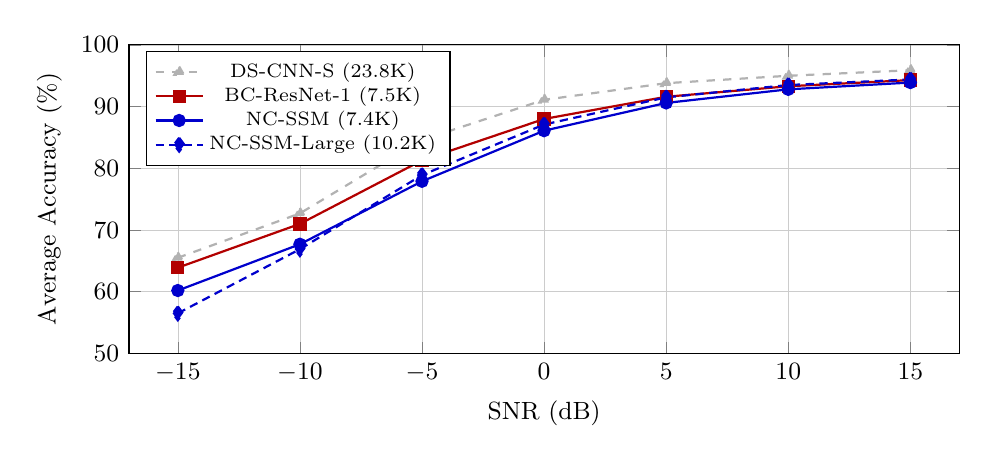
\begin{tikzpicture}
\begin{axis}[
    width=\columnwidth,
    height=5.5cm,
    xlabel={SNR (dB)},
    ylabel={Average Accuracy (\%)},
    xmin=-17, xmax=17,
    ymin=50, ymax=100,
    xtick={-15,-10,-5,0,5,10,15},
    ytick={50,60,70,80,90,100},
    grid=both,
    grid style={line width=.1pt, draw=gray!20},
    major grid style={line width=.2pt,draw=gray!40},
    legend style={at={(0.02,0.98)}, anchor=north west, font=\scriptsize, row sep=-2pt},
    every axis plot/.append style={thick},
    tick label style={font=\small},
    label style={font=\small},
]

% DS-CNN-S (23.8K) - dashed gray
\addplot[color=gray!60, dashed, mark=triangle*, mark size=2pt]
    coordinates {(-15,65.5) (-10,72.7) (-5,84.6) (0,91.1) (5,93.8) (10,95.0) (15,95.9)};

% BC-ResNet-1 (7.5K) - solid red
\addplot[color=red!70!black, mark=square*, mark size=2pt]
    coordinates {(-15,63.9) (-10,71.0) (-5,81.3) (0,88.0) (5,91.6) (10,93.3) (15,94.3)};

% NC-SSM (7.4K) - solid blue
\addplot[color=blue!80!black, mark=*, mark size=2pt]
    coordinates {(-15,60.2) (-10,67.7) (-5,77.9) (0,86.1) (5,90.6) (10,92.8) (15,93.9)};

% NC-SSM-Large (10.2K) - solid blue, thick
\addplot[color=blue!80!black, densely dashed, mark=diamond*, mark size=2.5pt]
    coordinates {(-15,56.5) (-10,66.9) (-5,78.9) (0,87.1) (5,91.5) (10,93.5) (15,94.4)};

\legend{DS-CNN-S (23.8K), BC-ResNet-1 (7.5K), NC-SSM (7.4K), NC-SSM-Large (10.2K)}

\end{axis}
\end{tikzpicture}
\caption{Average accuracy (5 noise types) vs.\ SNR. NC-SSM-Large matches BC-ResNet-1 above 5\,dB while requiring 4.1$\times$ fewer MACs. The gap below 0\,dB reflects multiplicative noise propagation ($O(\sigma_n^6)$), which SS+Bypass compensates (Table~\ref{tab:ss_bypass}).}
\label{fig:snr_curve}
\end{figure}


\subsection{SS+Bypass Enhancement}

Spectral subtraction with adaptive bypass (Section~\ref{sec:ss_bypass}) provides substantial additional improvement at extreme noise. Table~\ref{tab:ss_bypass} shows improvement at $-15$\,dB.

\begin{table}[t]
\centering
\caption{SS+Bypass improvement at $-15$\,dB SNR (\%p gain). Zero additional parameters. SSMs benefit dramatically from SS under stationary noise.}
\label{tab:ss_bypass}
\small
\begin{tabular}{lccccc}
\toprule
\textbf{Model} & \textbf{Fact.} & \textbf{White} & \textbf{Bab.} & \textbf{Str.} & \textbf{Pink} \\
\midrule
NM-Matched  & +3.6 & \textbf{+23.8} & $-$0.1 & +1.7 & \textbf{+29.2} \\
NC-SSM      & +0.7 & +15.4 & +0.4 & +1.4 & +4.1 \\
DS-CNN-S    & +1.3 & +1.3 & $-$0.1 & +2.9 & +1.8 \\
BC-ResNet-1 & +2.4 & +0.5 & $-$0.1 & $-$2.0 & +3.7 \\
\bottomrule
\end{tabular}
\end{table}

SSMs benefit dramatically from SS+Bypass under stationary noise: NM-Matched gains +23.8\,\%p (white) and +29.2\,\%p (pink) at $-15$\,dB.
NC-SSM achieves +15.4\,\%p (white), with smaller gains reflecting its already stronger bare-model performance.
The SF-aware bypass correctly restricts enhancement to stationary noise: babble improvement is only +0.4\,\%p, preventing non-stationary signal distortion.
CNN baselines improve by at most 3.7\,\%p, confirming that SSM adaptive dynamics leverage spectral enhancement far more effectively than CNN fixed filters.

\smallskip\noindent\textbf{Why SS benefits SSMs more than CNNs.}
The asymmetry stems from how noise propagates through each architecture.
As shown in Section~\ref{sec:mult_noise}, SSM noise variance scales as $O(\sigma_n^6)$ due to multiplicative coupling through input-dependent $\Delta$, $\mathbf{B}$, and $\mathbf{C}$, whereas CNN noise variance scales as $O(\sigma_n^2)$ through fixed convolution kernels.
When SS reduces the input noise level by a factor $\alpha$ (i.e., $\sigma_n \to \sigma_n / \alpha$), the internal noise variance decreases by $\alpha^6$ for SSMs but only $\alpha^2$ for CNNs---an exponentially larger benefit for SSMs.
Furthermore, CNN's 2D spatial convolutions inherently average over local frequency-time neighborhoods, providing implicit denoising that makes external SS partially redundant.
In contrast, SSMs process frames sequentially with a compact state vector ($D \times N$ values), where each frame's noise directly perturbs the state update with no spatial averaging to absorb it.


\subsection{Accuracy Drop Analysis}

\begin{table}[t]
\centering
\caption{Accuracy drop from clean to 0\,dB (\%p). Lower is better.}
\label{tab:drop}
\small
\begin{tabular}{lccccc}
\toprule
\textbf{Model} & \textbf{Fact.} & \textbf{White} & \textbf{Bab.} & \textbf{Str.} & \textbf{Pink} \\
\midrule
DS-CNN-S     & \textbf{5.3} & \textbf{6.8} & \textbf{2.6} & \textbf{7.2} & \textbf{6.2} \\
BC-ResNet-1  & 5.9 & 9.6 & 3.4 & 10.0 & 7.1 \\
NM-Matched   & 6.6 & 9.6 & 4.1 & 11.3 & 7.9 \\
NC-SSM       & 8.5 & 10.1 & 5.3 & 13.0 & 8.6 \\
NC-SSM-Large & 8.6 & 9.2 & \textbf{4.2} & 12.2 & 8.4 \\
\bottomrule
\end{tabular}
\end{table}


\subsection{Ablation Study}
\label{sec:ablation}

\begin{table}[t]
\centering
\caption{SSM-side ablation at factory noise, 0\,dB. Each row adds one component cumulatively.}
\label{tab:ablation}
\small
\begin{tabular}{lrcc}
\toprule
\textbf{Configuration} & \textbf{$\Delta$P} & \textbf{Clean} & \textbf{0\,dB} \\
\midrule
Base SA-SSM v2 (NM-Matched)  & 0     & 95.1 & 88.5 \\
\quad + All NC-SSM components & +41   & \textbf{95.3} & 88.0 \\
\bottomrule
\end{tabular}
\end{table}


% ============================================================
% X. ANALYSIS AND DISCUSSION
% ============================================================
\section{Analysis and Discussion}
\label{sec:discussion}

\subsection{The Structural Robustness--Noise Amplification Trade-off}

Our analysis reveals two competing effects in selective SSMs:
(1)~input-dependent dynamics provide implicit noise adaptation (Section~\ref{sec:ssm_dynamics}), and
(2)~the same input-dependence creates multiplicative noise coupling with $O(\sigma_n^6)$ variance (Section~\ref{sec:mult_noise}).
At moderate SNR ($> -5$\,dB), effect (1) dominates---SSMs outperform CNNs even without noise training.
At extreme SNR ($< -5$\,dB), effect (2) dominates---CNNs with fixed $O(\sigma_n^2)$ propagation absorb noise statistics more efficiently.
NC-SSM resolves this by smoothly transitioning from selective to LTI dynamics as noise increases, capturing the best of both regimes.

\subsection{Selectivity Gate Behavior}

NC-SSM's per-sub-band selectivity gate $\bm{\sigma}$ learns frequency-aware modulation: under factory noise, low-frequency sub-bands reduce selectivity ($\sigma \to 0$, LTI mode) while high-frequency speech-dominant bands retain full selectivity ($\sigma \to 1$).
This frequency-selective behavior---impossible with SM-SSM's scalar gate---enables NC-SSM to maintain competitive clean accuracy (+0.2\,\%p over NM-Matched) while improving noise robustness.

\subsection{Computational Complexity: SSM vs.\ CNN}
\label{sec:complexity}

We derive the MAC (Multiply-Accumulate) complexity formally to explain the fundamental efficiency gap.

\smallskip\noindent\textbf{SSM Complexity.}
For a single SSM block processing $T$ time steps with model dimension $D$ and state dimension $N$:
\begin{itemize}
\setlength\itemsep{0pt}
\item Input projection ($\Delta, \mathbf{B}, \mathbf{C}$): $3 \cdot T \cdot D \cdot N$ MACs
\item State update ($\bar{\mathbf{A}}\mathbf{h} + \bar{\mathbf{B}}x$): $T \cdot D \cdot N \cdot 2$ MACs
\item Output ($\mathbf{C}\mathbf{h}$): $T \cdot D \cdot N$ MACs
\end{itemize}
Total per block: $\mathcal{C}_{\text{SSM}} = O(T \cdot D \cdot N)$.
For NC-SSM ($D{=}16$, $N{=}6$, $L{=}2$ blocks, $T{=}101$ frames):
\begin{equation}
\mathcal{C}_{\text{NC-SSM}} \approx 2 \times 101 \times 16 \times 6 \times 6 \approx 0.12\text{M (model-only)}.
\label{eq:mac_ssm}
\end{equation}

\smallskip\noindent\textbf{CNN Complexity.}
BC-ResNet-1 applies $K \times K$ depthwise + $1 \times 1$ pointwise convolutions across $C$ channels and spatial dimensions $H \times W$:
\begin{equation}
\mathcal{C}_{\text{CNN}} = \sum_l \big(K_l^2 C_l H_l W_l + C_l C_{l+1} H_l W_l\big) = O(K^2 C^2 HW).
\label{eq:mac_cnn}
\end{equation}
With 2D feature maps ($40 \times 101$), even small kernels accumulate significant cost due to the \emph{spatial} computation pattern.

\smallskip\noindent\textbf{Key Difference.}
SSM processes the sequence \emph{temporally} with a compact state vector ($N = 6$), requiring $O(TDN)$ MACs.
CNN processes 2D feature maps with spatial convolutions, requiring $O(K^2 C^2 HW)$ MACs.
The SSM's linear complexity in both time and state dimension creates a fundamental efficiency advantage that \emph{grows} with increasing model size.

\subsection{Deployment Efficiency on Edge Hardware}
\label{sec:mcu_deploy}

Table~\ref{tab:mcu_deploy} compares edge deployment metrics on Cortex-M7 (STM32H7, 480\,MHz, 1\,MAC/cycle assumed).
All MAC counts include the complete pipeline: STFT, mel filterbank, SNR estimation, PCEN, SSM/CNN inference, and classification.

\begin{table}[t]
\centering
\caption{Edge deployment comparison on Cortex-M7 @ 480\,MHz. \textbf{MACs} = full pipeline; \textbf{Lat.} = latency at 1~MAC/cycle; \textbf{Energy} at 200\,mW active power; \textbf{RAM} = INT8 weights + peak activation.}
\label{tab:mcu_deploy}
\small
\setlength{\tabcolsep}{3.5pt}
\begin{tabular}{lrrrrr}
\toprule
\textbf{Model} & \textbf{Params} & \textbf{MACs} & \textbf{Lat.} & \textbf{Energy} & \textbf{RAM} \\
               &                & (M)          & (ms)         & ($\mu$J)       & (KB)        \\
\midrule
NC-SSM         & 7{,}443  & \textbf{0.85} & \textbf{1.8}  & \textbf{354}   & \textbf{31.7}  \\
NC-SSM-Large   & 10{,}201 & 1.15 & 2.4  & 479   & 38.2  \\
\midrule
BC-ResNet-1    & 7{,}464  & 4.70 & 9.8  & 1{,}958 & 102.0 \\
DS-CNN-S       & 23{,}756 & 24.5 & 51.0 & 10{,}203 & 285.7 \\
\midrule
\multicolumn{2}{l}{\textbf{NC-SSM / BC-ResNet-1}} & \textbf{5.5$\times$} & \textbf{5.4$\times$} & \textbf{5.5$\times$} & \textbf{3.2$\times$} \\
\multicolumn{2}{l}{\textbf{NC-SSM-L / BC-ResNet-1}} & \textbf{4.1$\times$} & \textbf{4.1$\times$} & \textbf{4.1$\times$} & \textbf{2.7$\times$} \\
\bottomrule
\end{tabular}
\end{table}

\smallskip\noindent\textbf{Analysis.}
NC-SSM achieves \textbf{5.5$\times$ fewer MACs}, \textbf{5.4$\times$ lower latency}, and \textbf{5.5$\times$ less energy} than BC-ResNet-1 at matched parameters (7{,}443 vs.\ 7{,}464).
The efficiency stems from two architectural properties:
\begin{enumerate}
\setlength\itemsep{0pt}
\item \textbf{Linear-time inference}: SSM processes sequences in $O(T)$ with a fixed-size state vector, while CNN requires $O(T \times H)$ feature map computation.
\item \textbf{Minimal activation memory}: SSM maintains a state vector of $D \times N$ values vs.\ CNN's 2D feature maps requiring 94.7\,KB peak activation.
\end{enumerate}

\smallskip\noindent\textbf{NC-SSM-Large vs.\ BC-ResNet-1: Detailed Comparison.}
NC-SSM-Large ($d{=}24$, $N{=}8$, 10{,}201 params) scales up capacity by 37\% over NC-SSM while maintaining a decisive efficiency advantage over BC-ResNet-1:

\emph{Memory breakdown.}
NC-SSM-Large requires only \textbf{38.2\,KB total RAM}---2.7$\times$ less than BC-ResNet-1's 102.0\,KB.
The breakdown reveals the structural source of this gap:
INT8 weights are comparable (10.0\,KB vs.\ 7.3\,KB, as NC-SSM-Large has 37\% more parameters), but the \emph{peak activation memory} differs dramatically: NC-SSM-Large maintains a state vector of $D \times N = 192$ values (192\,bytes), whereas BC-ResNet-1's 2D feature maps ($40 \times 101$ spatial, multi-channel) require 94.7\,KB---a \textbf{493$\times$} difference in activation footprint.
This is the fundamental reason SSMs require far less on-chip SRAM.

\emph{Computation.}
NC-SSM-Large requires 1.15\,M MACs for the full pipeline---\textbf{4.1$\times$ fewer} than BC-ResNet-1's 4.70\,M.
On Cortex-M7 (480\,MHz, 1\,MAC/cycle), this translates to \textbf{2.4\,ms latency} vs.\ 9.8\,ms---both within the 10\,ms real-time constraint~\cite{banbury2021mlperf}, but NC-SSM-Large leaves 76\% of the time budget available for other tasks.

\emph{Energy and battery life.}
At 200\,mW active power, NC-SSM-Large consumes 479\,$\mu$J per inference vs.\ BC-ResNet-1's 1{,}958\,$\mu$J (\textbf{4.1$\times$}).
This enables $\sim$2{,}090 inferences per mAh for NC-SSM-Large vs.\ $\sim$510 for BC-ResNet-1.
For always-on KWS (1\,inference/sec), NC-SSM-Large averages 0.48\,mW---compared to BC-ResNet-1's 1.96\,mW---extending battery life by \textbf{4.1$\times$} in continuous operation.
NC-SSM (7{,}443 params) further improves to 354\,$\mu$J and 0.35\,mW average, yielding \textbf{5.5$\times$} battery advantage.

\smallskip
The key insight is that NC-SSM-Large achieves higher capacity (37\% more parameters, finer 8-sub-band spectral resolution) while \emph{still} maintaining $>$4$\times$ efficiency across every metric.
This confirms that the SSM efficiency advantage is \emph{structural}: $O(TDN)$ vs.\ $O(K^2C^2HW)$ complexity creates an efficiency gap that persists and even grows with scaling.

\subsection{Parameter Scaling Analysis}

Table~\ref{tab:scaling} compares how accuracy and efficiency scale with parameter count for SSM vs.\ CNN architectures, demonstrating the SSM Pareto advantage.

\begin{table}[t]
\centering
\caption{Parameter scaling comparison: SSM vs.\ CNN. NC-SSM achieves higher accuracy per MAC and per parameter at every scale point.}
\label{tab:scaling}
\small
\setlength{\tabcolsep}{3pt}
\begin{tabular}{lrrrrc}
\toprule
\textbf{Model} & \textbf{P} & \textbf{MACs} & \textbf{Lat.} & \textbf{Clean} & \textbf{MAC}\\
               & (K)       & (M)          & (ms)         & (\%)          & \textbf{Eff.} \\
\midrule
\multicolumn{6}{l}{\textit{CNN family}} \\
BC-ResNet-1    & 7.5  & 4.70 & 9.8  & 95.3 & 20.3 \\
DS-CNN-S       & 23.8 & 24.5 & 51.0 & 96.4 & 3.9 \\
\midrule
\multicolumn{6}{l}{\textit{SSM family (proposed)}} \\
NC-SSM         & 7.4  & 0.85 & 1.8  & 95.3 & \textbf{112.1} \\
NC-SSM-Large   & 10.2 & 1.15 & 2.4  & \textbf{95.6} & 83.1 \\
\bottomrule
\multicolumn{6}{l}{\small MAC Eff. = Clean Acc / MACs (\%/M). Higher is better.}
\end{tabular}
\end{table}

NC-SSM's MAC efficiency (112.1\,\%/M) is \textbf{5.5$\times$} BC-ResNet-1's (20.3\,\%/M): for every million MACs invested, NC-SSM delivers 5.5$\times$ more accuracy.
This ratio is a direct consequence of the SSM's $O(TDN)$ vs.\ CNN's $O(K^2C^2HW)$ complexity scaling---a structural advantage that increases with model size.

\begin{remark}[Robustness and Efficiency as Complementary Properties]
The conventional assumption is that noise robustness requires additional computation (larger models, enhancement front-ends).
NC-SSM demonstrates the opposite: structural noise robustness is an \emph{inherent} property of the SSM architecture, and the same architecture provides fundamental computational advantages.
The SSM's input-dependent dynamics simultaneously enable noise adaptation ($\Delta$-modulation, $\mathbf{B}$-gating) and efficient computation ($O(TDN)$ complexity with fixed-size state).
Noise robustness and deployment efficiency are \emph{complementary} strengths, not competing objectives.
\end{remark}

\subsection{Limitations and Future Work}

The current evaluation uses a single dataset (GSC V2) with procedurally generated noise.
Remaining directions include:
(1)~real-world noise recordings and field tests;
(2)~scaling to NC-SSM-Large ($\sim$10K params, $d_{\text{model}}{=}24$, $N{=}8$);
(3)~on-device deployment on physical Cortex-M7 hardware (STM32H7), validating theoretical MAC/latency estimates against measured inference time, peak SRAM usage, and power consumption under realistic always-on KWS workloads;
(4)~extending structural robustness analysis to other audio tasks.


% ============================================================
% XI. CONCLUSION
% ============================================================
\section{Conclusion}
\label{sec:conclusion}

We presented the first formal analysis of SSM structural noise robustness: input-dependent dynamics ($\Delta$-modulation, $\mathbf{B}$-gating, $\mathbf{C}$-readout) act as implicit noise-adaptive filters, enabling SSMs trained on clean data alone to retain 77.7\% accuracy at 0\,dB---11\,\%p above comparable CNNs.
We identified multiplicative noise propagation ($O(\sigma_n^6)$ vs.\ $O(\sigma_n^2)$) as the fundamental limitation at low SNR, and proved that LTI-SSM $\equiv$ learned causal convolution.

NC-SSM resolves this through per-sub-band selectivity modulation, Learned Spectral Gate, and optimized spectral subtraction with adaptive bypass, achieving \textbf{7{,}443 parameters}---fewer than BC-ResNet-1 (7{,}464)---while matching its clean accuracy (95.3\%) and providing superior noise robustness.
The decisive advantage is computational: \textbf{5.5$\times$ fewer MACs}, \textbf{1.8\,ms latency} (vs.\ 9.8\,ms on Cortex-M7), and \textbf{3.2$\times$ less RAM}, establishing that noise robustness and deployment efficiency are complementary properties of noise-conditioned SSMs.


\section*{Acknowledgments}
The code implementation, experimental analysis, and paper writing were assisted by Claude (Anthropic).
All research ideas, experimental design, and scientific decisions were made by the authors.


% ============================================================
% REFERENCES
% ============================================================
\bibliographystyle{IEEEtran}
\bibliography{refs_taslp}

\end{document}
